
\documentclass[conference]{IEEEtran}

\usepackage{graphics}
\usepackage{epsfig}
\usepackage{epstopdf}

% *** GRAPHICS RELATED PACKAGES ***
%
\ifCLASSINFOpdf
  % \usepackage[pdftex]{graphicx}
  % declare the path(s) where your graphic files are
  % \graphicspath{{../pdf/}{../jpeg/}}
  % and their extensions so you won't have to specify these with
  % every instance of \includegraphics
  % \DeclareGraphicsExtensions{.pdf,.jpeg,.png}
\else
  % or other class option (dvipsone, dvipdf, if not using dvips). graphicx
  % will default to the driver specified in the system graphics.cfg if no
  % driver is specified.
  % \usepackage[dvips]{graphicx}
  % declare the path(s) where your graphic files are
  % \graphicspath{{../eps/}}
  % and their extensions so you won't have to specify these with
  % every instance of \includegraphics
  % \DeclareGraphicsExtensions{.eps}
\fi
% graphicx was written by David Carlisle and Sebastian Rahtz. It is
% required if you want graphics, photos, etc. graphicx.sty is already
% installed on most LaTeX systems. The latest version and documentation
% can be obtained at: 
% http://www.ctan.org/pkg/graphicx
% Another good source of documentation is "Using Imported Graphics in
% LaTeX2e" by Keith Reckdahl which can be found at:
% http://www.ctan.org/pkg/epslatex
%

\hyphenation{op-tical net-works semi-conduc-tor}


\begin{document}

\title{Discovering Activities and Working Patterns in Developer Usage Data}



\author{\IEEEauthorblockN{Luis C. Cruz, Victor M. Gonzalez}
\IEEEauthorblockA{Instituto Tecnologico Autonomo de Mexico (ITAM)\\
Mexico City, Mexico}
\and
\IEEEauthorblockN{Romain Robbes}
\IEEEauthorblockA{Computer Science Department (DCC)\\
University of Chile, Santiago, Chile}}



% use for special paper notices
%\IEEEspecialpapernotice{(Invited Paper)}




% make the title area
\maketitle


\begin{abstract}
Software developers often perform multiple tasks throughout a day of work that involves developing new features, bug fixing, design, collaboration with other developers and much more. In this paper we identified developers' activities reflected in usage data from two sources and the patterns followed in working sessions using clustering techniques. We found several types of activities and patterns in accordance with observational studies and some differences between sources that reflect the different profiles of developers.
\end{abstract}

% no keywords




% For peer review papers, you can put extra information on the cover
% page as needed:
% \ifCLASSOPTIONpeerreview
% \begin{center} \bfseries EDICS Category: 3-BBND \end{center}
% \fi
%
% For peerreview papers, this IEEEtran command inserts a page break and
% creates the second title. It will be ignored for other modes.
\IEEEpeerreviewmaketitle



\section{Introduction}
The search for better working conditions in software engineering has been a research topic for many years now. From compilers and tools to methodologies and practices, there are a considerable amount of proposals of artifacts meant to assist in some part of the software development life cycle. But before that there is a discovery phase where researchers identify the parts-to-be-enhanced; it usually involves experiments, observational studies and/or surveys. Through those empirical analyses we are able to better understand how software engineering teams work and what kind of problems they face.

In order to understand developers' activities and practices, researchers resort to observational studies, experiments and surveys to extract the data \cite{LVD06, KMC06, GM04, PR11}. Another way to do this is by analyzing usage data, that contains the history of interactions between the developer and development tools or IDEs (Integrated Development Environment). With this information we can tell how other events (like work fragmentation \cite{SRV15}) affect the activity of the developers \cite{SnipesETALASD}. Analyzing this kind of data is part of the Mining Software Repositories research area \cite{H04} and it is often used to understand how developers work.

The objective of this work is to extract knowledge from interaction data between developers and IDE that allows us to understand the amount of information reflected in it about the programmers' activities. Specifically, the objective is to answer the following research questions:
\begin{itemize}
	\item RQ1: What kind of activities can be identified with interaction data?
	\item RQ2: What working patterns during a session are commonly performed by developers?
\end{itemize}

In the next Section we describe some of the related work about developers' activities and usage data. In Section 3 we describe the two datasets used in this work. In Section 4, we describe some of the initial phases of the methodology that contain the pre-processing and transformation of the datasets. In Section 5 we give details about our approach to discovering the activities and comment on the results. Based on the results on the discovery of activities, in Section 6 we inquiry about the patterns of working sessions. In Section 7 we analyze the validity of the results and we finish with concluding remarks in Section 8.
\section{Related Work}
In recent years there has been a lot of effort in understanding the way developers work and the challenges they face. With that information we can design tools \cite{CD10, P14, CLQ15, KM06} that offer better conditions on everyday activities. 

Singel et al. \cite{SLV10} surveyed developers to get information of common work practices. They found that programmers spend about half of the time writing code and attending to meetings, and a third or less of the time doing research, configuring, fixing bugs, designing and testing. When shadowing software engineers they were able to get several categories for the activities performed. Similarly, LaToza et al. \cite{LVD06} defined a category of activities related to code and motivation; the difference between both classifications is that the latter considers collaboration activities with other developers.

Baracchi \cite{B14} analyzed four kinds of programmer's activities: understanding, editing, inspection and navigation. His findings indicate that the edition activities can be only 20\% of a working session and understanding more than 70\%. Moreover, he classified the working sessions in four groups: Enhancement, Bug-fixing, Refactoring and General. Enhancement sessions are the most common and are followed by the General purpose type of sessions. He uses interaction data with the IDE (Integrated Development Environment).

Program understanding (referred also as program comprehension) involves all kinds of activities meant to better understand the code in development, like reading the code and documentation, follow a problem-solution-test pattern, interacting with the UI (User Interface), debugging the application, taking notes and more techniques according to Roehm et al. \cite{RTK12}. According to Rugaber \cite{R95}, the difficulty of program comprehension lies in its objective of bridging different concepts. It is an activity that covers a considerable working time of a developer, as observed in multiple studies \cite{FH83, BGZ15, B14, MMLK14}.

About testing tasks, Beller et al. \cite{BGZ15} developed a tool to extract usage data from the IDE in order to study the testing practices of software developers. They found that on average they spent 9\% the time testing code, but it can get well below that percentage. Also, developers execute about 5 tests per day roughly every 50 minutes.

Murphy et al. \cite{MKF06} analyzed usage data of multiple programmers with the Eclipse IDE. They found that some of the most commonly executed commands are delete, save, next word and paste. Also, they found that programmers use 11 kinds of refactoring commands (e.g. rename, move, extract and pull up); these commands are often executed via key bindings and exploring the menus.

On refactoring activities, Murphy-Hill et al. \cite{MPB12} used the Eclipse Usage Data Collector dataset to understand how programmers are using refactoring tools analyzing the patterns of refactoring practices, finding that most programmers do not make deep use of these tools, leaving untouched most of the configuration parameters and performing manually most of the refactoring.

The core of this work is within the Mining Software Repositories research area, which can be defined as the extraction of information from different artifacts (e.g. source code, control version logs, documentation and bug reports) that are produced throughout the software development cycle \cite{H04}. This term is not alien to data mining, so the intentions are extracting knowledge and discovering patterns in the data using a set of techniques and algorithms for this goal \cite{FPG96}.

An example of data that can be captured is the usage data (also called interaction data) between the programmer and the development tools \cite{SnipesETALASD}, which are basically a log of the execution of events within the IDE. With usage data, Kersten and Murphy \cite{KM06} proposed a tool that keep the context of the task being performed by the programmer and make it visible to help in the navigation around elements. Fritz et al. \cite{FMH07} did a research about the possibility of inferring weather the programmer has knowledge of the code or not by quantifying the degree of interest. Carter and Dewan \cite{CD10} inquire about the possibility of identifying a programmer stuck or having problems. Minelli et al. \cite{MMLK14} performed an analysis about the process of program comprehension and compared the results with the literature. Sanchez et al. \cite{SRV15} used interaction data to perform an empirical analysis of the impact of work fragmentation on productivity.

\section{Description of the Data}
The results presented in this work are based on the information that can be extracted from usage data. We used two datasets to provide answers to our research questions that come from different sources but are similar in the kind information contained. 

It is important to first describe the data in terms of the attributes, magnitude and context of extraction. In the following subsections we describe in detail the characteristics of the datasets, limitations and some inferences we can obtain.

\subsection{Eclipse Usage Data Collector}
The Usage Data Collector is a large dataset containing usage data from users of Eclipse, extracted from December 2008 to August 2010; the objective was to get insight of how developers are using the IDE. The tool keeps track of the events triggered by the developer or the IDE itself. The kind of events captured include edition and navigation commands; the startup of plug-in and bundles; events invoked from menu or tool-bars, perspective changes and more. The dataset contains 2,323,233,101 unique rows (events) with 5 attributes. The information comes from approximately 1,800,000 users. The Table \ref{tbl:att_udc} shows a description of the attributes.

This dataset only contains information of the execution of commands within the IDE and we do not have more context about the programmers or environments. Judging by the registry of events, there is a mix of programmers of different nature like Java SE, Java EE and Web developers. There are also programmers that use other kind of languages like PHP, SQL and Ruby. We assume that this data corresponds to programmers of all levels of expertise, from students to professionals.


\begin{table}[ht!]
	\small
	\caption{Attributes of the UDC dataset. }
	\label{tbl:att_udc}
	\centering
	\begin{tabular}{|p{1.5cm}|p{5cm}|} 
		\hline 
		\emph{Attribute} & \emph{Description} \\  
		\hline 
		\hline 
		UserId &  Unique number that identifies a user \\
		\hline
		What & The action of the event (deactivated, activated, opened, executed, etc.)  \\
		\hline
		Kind & What kind of event was executed (workbench, view, command, etc.)  \\
		\hline
		BundleId & Description of the event's package  \\
		\hline
		BundleVersion & Version of the bundle's event  \\
		\hline
		Description & Description of the event\\
		\hline
		Datetime & Date and time in UNIX format\\
		\hline
	\end{tabular}
	
\end{table}

We used a version of the data that is published on Google BigQuery, by Murphy-Hill et al. \cite{SnipesETALASD}, so the processing of the data is simple. We took a sample of the data from 1,000 random users. We ignored the attributes BundleId and BundleVersion and some events executed by the system. From this query we extracted 4,321,349 unique events

\subsection{Codealike and ABB}
Codealike \cite{CLQ15} is a tool that monitors the activity of the user and later offers analytics and insight about the programmer's productivity and working patterns. This tool is installed in the IDE (Eclipse and Visual Studio) and listens to the events executed by the user and system, similar to UDC. It captures almost the same kind of events like edition, navigation and tool usage. Shortly after the capture of events, the user can observe information derived from his activity through a website.

Corvalius (the Argentinian company that created Codealike) is collaborating with ABB, a multinational corporation operating mainly in robotics, power and automation technology areas. The ABB's Software Engineering Research Group is using Codealike to obtain information from its developers with the objective of improving productivity and software quality. We had access to a dataset corresponding to the monitoring of 87 programmers between May and October of 2015 comprising 15,597,697 unique events. The main dataset that contains the registry of executed commands has the attributes described in the Table \ref{tbl:att_abb}.

The data was extracted from Visual Studio via Codealike and the events seems to correspond to .NET programming languages, like C\# or Visual Basic. Similar to UDC, it only contains a registry of executed commands and no information about the developers, except for the country of origin judging by the email domain that was provided. The programmers were invited to use Codealike at will, so the amount of data collected varies among users. Additionally, we had access to the \emph{focus} level of the user, a feature of Codealike that measures the focus or concentration of programmers based on the amount of activity registered within the IDE. We assume that this data corresponds to professional programmers working for the same company and under similar circumstances. The latter meaning that they all have the same or similar equipment, methodology, tools and working hours. However, we can not be certain about any of these assumptions.

\begin{table}[ht!]
	\small
	\caption{Attributes of the ABB dataset. }
	\label{tbl:att_abb}
	\centering
	\begin{tabular}{|p{1.5cm}|p{5cm}|} 
		\hline 
		\emph{Attribute} & \emph{Description} \\  
		\hline 
		\hline 
		Username &  Unique identifier of the user \\
		\hline
		Timestamp & Date and time of the execution  \\
		\hline
		Event & Identifier of the event's description  \\
		\hline
		Category & Unique identifier of the event's category \\
		\hline
	\end{tabular}
	
\end{table}

The actual description of the events is stored on a different file, so we use the values of the Category and Events attributes to extract it. In this case, all the attributes are needed. From hereafter this dataset will be referred as ABB.

\section{Methodology}
We followed the steps described by the \emph{Knowledge Discovery in Databases} process \cite{FPG96}, a set of iterative steps composed of Selection, Preprocessing, Transformation, Data Mining and Interpretation. The Selection was covered by the last section and the following sections will describe the tasks performed during the Preprocessing and Transformation steps. In the latter sections we will give details about the Data Mining and Interpretation steps.

\subsection{Preprocessing}
During the Preprocessing stage we performed mainly two tasks: data cleaning and classification. The cleaning tasks are trivial, for the data is in overall good shape. However classifying the events is a complicated task that requires careful inspection and multiple iterations. The tasks involving data cleaning diverge between datasets, so we give details about this step separately. But the classification of events follows the same process for both datasets and is described afterwards.

\subsubsection{UDC}
First, we added an attribute with the time elapsing between one event and the next one and an ID to identify the different working sessions present on the data. For the latter, we sorted the data by UserId and Datetime. This was required because, by default, the user's data is mixed and we need it not only chronologically correct but also sorted by users to tag the working sessions of every user without interferences. We also filled the description for the events that indicate the activation or deactivation of the Eclipse's workbench, which were the only ones with that issue.

\subsubsection{ABB}
The Preprocessing for ABB is also simple. As with UDC, we added a duration in seconds and an ID to every event. Then, we extracted the Description from a second dataset, according to the Event and Category, and created a new attribute. We changed the Description to lowercases and removed curly braces and other special characters. 
An interesting feature of this dataset is that plenty of data seems to be somewhat systematic, with a certain event executed every 5 minutes or less. We do not know in what scenarios this kind of activity is recorded (it could be executed by the IDE) so we decided to remove those observations. Finally, we ordered the data by Username and Datetime.

\subsection{Classification of events}
To classify the events, we look into the description to see what it can tell us about the event. It is based on activities found in the literature and the data we have available. We describe the classification in the Table \ref{tbl:detailed_events}.

\begin{table*}[ht!]
	\caption{Description of the classification of events. }
	\label{tbl:detailed_events}
	\centering
	\begin{tabular}{|p{2cm}|p{6cm}|p{5.5cm}|} 
		\hline 
		\emph{Classification} & \emph{Description} & \emph{Examples} \\  
		\hline 
		\hline 
		Edit-Text &  Text edition events & Copy, Paste and Delete. \\
		\hline
		Text-Nav & Events executed when navigating around text. & LineUp, LineDown and LineEnd.  \\
		\hline
		High-Nav & Navigation of high level, like around classes and views. & GoToDefinition, NextTab and GoToSuperclass \\
		\hline
		Debug & Events executed during debugging sessions. & StepInto and StepOver. \\
		\hline
		Search & Events executed when searching for objects and text. & Search, Find and FindReplace. \\
		\hline
		Refactoring & Events executed when restructuring code. & Encapsulate, Rename and MoveField. \\
		\hline
		Testing & When testing (e.g. unit tests) is executed through a framework. & ExecuteTest and TestResults. \\
		\hline
		Control & Execution of version control tasks. & Compare, ViewChanges and CommitChanges. \\
		\hline
		Clean-Build & Tasks performed by the IDE to build and execute a solution.  & Build and Run. \\
		\hline
		File & Events executed during the management of files. & Open, Close and SaveChanges. \\
		\hline
		Tools & Execution of specialized tools and plugins. & DatabaseDesigner, Codealike and UIDesigner.\\
		\hline
	\end{tabular}
	
\end{table*}

To assign a type to every event we use the description. In both datasets the description has the format \emph{path.to.class.ListenerClass}. It contains the path to the class that works as listener of the event and executes the required task. The packages and class name give out information about the nature of the event.

With that in mind, we created a set of rules that adds a classification to every event according to the name of the class and/or the name of the path. For example, in UDC we label as Text-Nav all the events that have \emph{ui.edit.scroll} in the description, and in ABB we label as High-Nav all the events whose class name is \emph{NextTab}. Sometimes it was required to create special rules for certain events but most of the time we were able to set rules for several of them. This was an iterative process that required careful inspection of the results.

\subsection{Transformation}
From the Transformation phase and on, the activities are the same for both datasets. The objectives of the transformation phase are identifying the working sessions and calculating a set metrics and time series for each. Then every session is decomposed into chunks or segments of smaller time than sessions.


To identify working sessions we look for interruptions of work (or a pause of the recorded activity) that last for more than 4 hours, similar to \cite{SRV15}. Any segment of activity surrounded by interruptions with that duration is labeled as a session. However, in order for the segment to be valid it must be of at least 30 minutes of duration.

Then, for every session we created several time series representing the execution of events by classification. Taking the minute as time unit, we counted the number of events executed on every minute and created eleven time series, where the amplitude is the number of events. 

After that, the next step is to calculate the proportion of events by type, which is the count of events by every type divided by the total of events executed in the session. There are a total of 11 values for this metric.

The last task of the transformation phase is to split the sessions into smaller activity frames to do analyses of the programmer's activity in detail. For that we split the time series of every session into time segments of 3 to 5 minutes of continuous activity that we will call chunks. It was necessary to recreate the time series and proportions for the chunks. After this, every user has a set of sessions (with their respective time series) and every session has a series of chunks.

We can observe some statistics about the resulting sessions in the Table \ref{tbl:stats_sessions}. UDC contains much more sessions, but in average they are shorter (4.11 hrs) than the sessions in ABB (7.33 hrs). However, in both cases the actual time spent working in the IDE is much less, being in average of 64.29 minutes for UDC and 166.08 minutes in ABB. The average number of interruptions per session is larger in ABB (25.40) than in UDC (9.52), which is in relation to the size of the sessions, but in ABB the interruptions tend to be shorter (10.74 minutes).

\begin{table}[ht!]
	\small
	\caption{Statistics of sessions in UDC and ABB. }
	\label{tbl:stats_sessions}
	\centering
	\begin{tabular}{|p{3.5cm}|p{2cm}|p{2cm}|} 
		\hline
		\emph{Statistic} & \emph{UDC} & \emph{ABB} \\
		\hline
		\hline
		Number of sessions & 6,405 & 1,182 \\
		\hline
		Number of observations & 2,848,270 & 2,449,227 \\
		\hline
		Number of users & 621 & 69 \\
		\hline
		Number of chunks & 43,769 & 23,624 \\
		\hline
		Avg. duration & 4.11 hrs. & 7.33 hrs. \\
		\hline
		Avg. productive time & 64.29 min & 166.08 min \\
		\hline
		Avg. of interruptions & 9.52 & 25.40 \\
		\hline
		Avg. duration of inte. & 18.94 min & 10.74 min \\
		\hline
	\end{tabular}
\end{table}

\section{Discovering Activities}

In the literature we can find evidence about the kind of activities performed by programmers, mostly from observational studies and usage data \cite{LVD06, GM04, MMLK14, MKF06}. We could have defined a set of activities based on the conclusions from these resources, but how can we assure that the same activities are present in our data? Do we have enough data to identify those activities? Is the same kind of activities identifiable in both datasets? These are some of the problems in establishing a set of activities based on related work. To avoid that we used clustering techniques to find them. This way we can find a set of common activities according to the data and the thresholds to differentiate between them.

During the Transformation phase we obtained a set of sessions and decomposed each into chunks of smaller size. Moreover, every one of these chunks has the proportion of execution of events by every type of the classification. So, the observations that were clustered are chunks and the attributes are the proportions. This means we have two datasets with 43,769 (UDC) and 23,624 (ABB) observations with 11 numerical attributes each.

As we do not know the number of activities we need an algorithm that chooses the number of clusters based on the data provided, like Mean Shift, Affinity Propagation and DBSCAN. We need an implementation that allows us to explore the values for each of the axis (attributes) of the found clusters, so we only considered Mean Shift and Affinity Propagation.

Mean Shift \cite{CM02} discovers centers based on the density of samples of a set of regions whose size relies on the parameter $bandwidth$. It updates possible centroids so they are mean of the samples within a given region. Afterwards, the centers that are near-duplicate are summarized and then it presents the final set of centers. After some initial experiments, the results with this algorithm tend to contain a small number of clusters; it finds very common activities but ignores some rare that are absorbed by more general clusters. This is reflected in low average values of the distance within clusters, which is translated into bad Silhouette Coefficients, a metric described later.

Affinity Propagation \cite{FD07} creates clusters by sending messages between all the data points; this message contains a value indicating how suitable is a point to be an exemplar, and the accumulated values of the messages are used to make a decision. This is performed until high-quality exemplars are found and corresponds to a cluster. We observed after some experiments that this algorithm tends to create a high number of clusters, providing all kinds of activities but some of them at many levels; this means that several clusters cover one activity (e.g. Programming) but at different levels of intensity (e.g. high usage of Programming and low usage of Programming). This can be seen as the contrary effect of the Mean Shift results and also with bad Silhouette averages. The main drawback of this algorithm is the high time-complexity of the order $O(n^2t)$, where $n$ is the number of samples and $t$ the number of iterations.

The Silhouette Coefficient \cite{R87} is a value per data point where high values are obtained from well defined clusters. It is composed of two scores: $a$ representing the mean distance between a sample and all other points of the same cluster, and $b$ the mean distance between a sample and all other points in the next nearest cluster. So, the Silhouette Coefficient $s$ of a point is obtained as:

$$s = \frac{b-a}{max(a,b)}$$

This coefficient evaluates the compactness (how close are objects within the same cluster) and separation (how well-separated is a cluster from other clusters). It is a value between -1 and 1; a value of 1 indicates that the point is correctly clustered and a -1 indicates that it is probably contained in the wrong cluster. Values around 0 means the observation lies between two clusters. We use the average Silhouette Coefficient (also known as the Silhouette width) to compare between models and to conclude if there is an actual structure in the data.

The issues of implementing only one clustering technique were solved with the following approach:

\begin{enumerate}
	\item First, cluster the observations with K-means into $k$ clusters. The parameter $k$ should be considerably big.
	\item Then cluster the resulting centroids with Mean Shift selecting a bandwidth $b$.
	\item Finally, label the observations according to the centroids of the second model.
\end{enumerate}

By clustering first with K-means we approximate the number of clusters with an algorithm with lower time-space complexity. The value for $k$ should be many times greater than the actual number of centers we expect to see. With this we try to cover all the probable activities, common and rare. The resulting clusters will be separated enough (and without much elements in between) so that they will not be summarized into one or two when applying the second clustering algorithm.

We still do not know what kind of activities are present in the data, so we need an algorithm that helps us discover them. For that, we cluster the centroids obtained from K-means with Mean Shift choosing a bandwidth $b$. To set the values for $k$ and $b$ we selected those that maximize the average Silhouette width. For ABB the parameters that maximize the metric are $k=3000$ and $b=0.41$. And for UDC the parameters should be $k=2500$ and $b=0.33$. With this approach we not only obtained acceptable clusters in terms of the activities they represent, but also got models with the best Silhouette width.

After we have the centers from Mean Shift, the next step is to add a label to each of them considering the values of the attributes. We took advantage that a high value for one of the attributes indicates that the activities of that center have heavy use of that event. Every center has a group of attributes with higher values than the rest; for example, a center labeled as Debugging has a value of 0.8 for the Debug attribute, and a value close to 0 for the rest, and a center labeled as Programming has higher values for the Edit-Text and Text-Nav attributes. The task involves manual work and the interpretation from the authors of what activity a cluster is modeling, so this could be a threat to the validity of the results. 

The assigned label represents the activity that a center models and several centers could represent the same activity. The Table \ref{tbl:activities} shows the resulting activities for ABB and UDC.

\begin{table}
	\caption{Activities found via clustering for UDC (left) and ABB (right).}
	\label{tbl:activities}
	\centering
	\begin{tabular}{| c | c |}
		\hline 
		\emph{Activity} & \emph{\% of chunks}\\  
		\hline 
		\hline
		Programming & 43.41 \% \\
		\hline
		Navigation & 38.05 \%\\
		\hline
		Debugging & 6.69 \% \\
		\hline	
		Tool-usage & 4.27\% \\
		\hline
		File-mgmt & 3.80 \% \\
		\hline 		
		Version & 2.88 \%\\
		\hline
		Search & 1.16 \% \\
		\hline
		Refactoring & 0.47 \% \\
		\hline
		
	\end{tabular}
	\quad
	\begin{tabular}{| c | c |}
		\hline 
		\emph{Activity} & \emph{\% of chunks}\\  
		\hline 
		\hline 
		Debugging & 44.45 \% \\
		\hline
		Programming & 34.67 \% \\
		\hline
		Navigation & 17.20 \%\\
		\hline
		Version & 2.77 \%\\
		\hline
		Tool-usage & 0.54 \% \\
		\hline
		Testing & 0.37	 \% \\
		\hline
	\end{tabular}
\end{table}

\subsection{Comparing activities between datasets}

Five activities (Programming, Navigation, Versioning, Debugging and Tool-usage) are present in both datasets and the rest are unique. We can see more variety of activities in the UDC dataset, which we attribute to the different types of programmers and to the sort of events that can be captured from the IDEs.

There are some interesting differences. First, the Programming activity is common in both cases with a high percentage of activities (43.41\% in UDC and 34.67\% in ABB), which agrees with other observational studies \cite{SLV10,LVD06} Surprisingly Debugging is only common in ABB (44.45\%), falling to the third place in UDC with only 6.69\%. Both datasets contain a very similar amount of events classified as Debug, that is 68 for UDC and 76 for ABB. The common events of control like start debugging, step over and step into are present in both datasets, but the problem is in the 8 extra events available in ABB. 

The ABB programmers, which are Visual Studio users, make heavy use of the Locals Window of Visual Studio that allows them to explore the state of the objects when debugging and change around processes and threads. Eclipse has a similar functionality in the Debug Perspective and captures an event when the programmer use it, but it does not support exploring different instances in the same fashion as Visual Studio. On top of that, in the ABB data the most common events of the type Debug are in fact those that allow to change the current process or thread. This could be the main cause for the differences of Debugging activities between datasets.

Another difference is that Navigation and Tool-usage activities have more incidence in the UDC data. First, in respect to Navigation, UDC users seems to perform more navigation around tabs and search for classes from the Package Explorer of Eclipse, also noted by Murphy et al. \cite{MKF06}. In the other hand, ABB users commonly perform navigation around the hierarchy of classes by calling to definitions. The kind of navigation performed by UDC users is translated into much more navigation events of high level and it is referred as unstructured navigation \cite{AFQ15}.

The amount of Tool-usage activities is related to the variety of programmers in the UDC data in contrast with ABB. In the former there are a group of users that are Web developers and execute events involving PHP, JavaServer Faces, HTML and CSS. To a lesser extent, there are also SQL and J2EE (Java Enteprise Edition) developers. In ABB the small amount of Tool-usage activities is mostly related to the design of classes and architecture of the system in development, and also to connections to SQL databases. From this, we can infer that the programmers in ABB have mostly \emph{back-end} roles and probably maintain an existing system that is supported by a multithreading paradigm, judging by our observations on the Debugging activities. However, we are unable to ascertain these assumptions.

Testing activities does not make an appearance in UDC and in ABB are present with a very low percentage. There are several ways of testing the code, some of them doing it by debugging and printing values or using a framework to create unit tests. Only events related to the latter can be observed in both datasets and it seems it is a rare way to do so. Moreover, Beller et al. \cite{BGZ15} observed that testing tasks are rare, with below 9\% of the working time of developers.

\section{Discovering Working Patterns}

During a working session, a programmer could go throughout several states or perform multiple activities. It might be possible to understand better this activities by using the information of the clusters we got in the previous subsection. 

In this section we look for patterns of sets of activities (sessions) that might be common among programmers. Due to the nature of the data we expect to see more common patterns in the ABB data and more variety in the UDC data, for more kind of programmers are present in the latter.

Once we had the chunks clustered and labeled, we divided the chunks of each session into three groups of equal size representing the beginning, middle and end. We selected 4 activities that are present in both datasets (Programming, Navigation, Debugging and Version), to facilitate the comparison, and calculated the proportion of each at every phase. After that, every observation (session) had 12 attributes and proceeded to cluster them using the Affinity Propagation technique; this time we want to see all the possible clusters without limiting to a low number like when clustering with chunks. 

We found 47 clusters in ABB and 98 in UDC, but we only work with the 5 more populated. The Figure \ref{ABB_phases} shows the results for ABB and UDC. The Types (A to E) are ordered from the most to the less populated. This selection covers 35\% of the sessions in ABB and 39\% in UDC. 

\subsection{Comparison of working session patterns}
For the sessions in ABB we have the following observations:
\begin{itemize}
	\item The most common pattern (Type A) involves mostly Debugging activities throughout the session and its followed by Type B, where the most common activity is programming throughout the session as well; it could be an effect of the two more frequent activities.
	
	\item The pattern described by the Type C is mostly composed of Navigation activities followed by Debugging. This can be related to program comprehension sessions \cite{MMLK14} or bug fixing due to the low amount of Programming.
	
	\item Types D and E have a fair amount for all the activities throughout the sessions and do not show notorious changes. Also, both Debugging and Programming are executed frequently, whence we relate these two patterns to multitasking sessions \cite{SLV10}.
	
	\item Versioning tasks are common during all the session when Programming is also a common. However it is only common at the begging or ending of the session when the Programming tasks are low. It could be that during Programming activities the user reaches more checkpoints that should be committed. 
\end{itemize}

For the sessions in UDC we have the following observations:
\begin{itemize}
	\item We relate Types A, C and D to multitasking sessions. The activities do not suffer sudden changes on any of the three phases.
	
	\item Type B keeps a steady amount of Programming throughout the session and there is a gradual increase of Debugging and Navigation until reaching a peak at the end. This is an interesting pattern that could be related to an increase of testing and proof of concept towards the end of the session.
	
	\item The sessions with a pattern of the Type E lacks completely of Debugging activities, while Programming is very common. Navigation and Version are only common at the beginning and end. This kind of sessions could be related to novice Programmers that instead of performing Debugging activities usually print to screen certain values to inspect the behavior of the program, also called tracing \cite{MKM08, AEH05}.
	
	\item Although Debugging is a rather uncommon activity, it is frequently executed (to some extent) during the most common working session patterns.
\end{itemize}
\begin{figure*}[!ht]
	
	\centering
	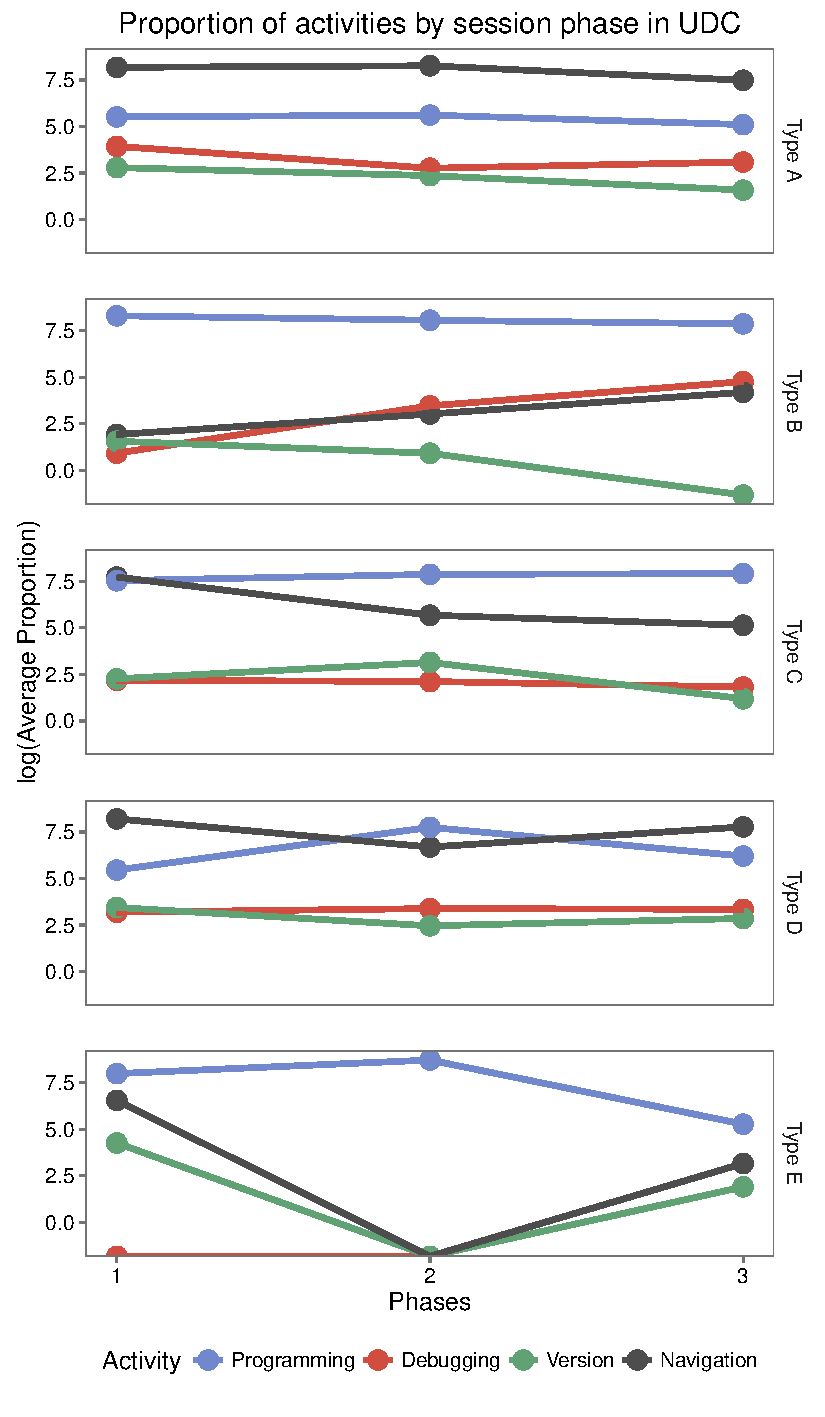
\includegraphics[width=0.35\textwidth]{Figures/UDC_phases_log}
	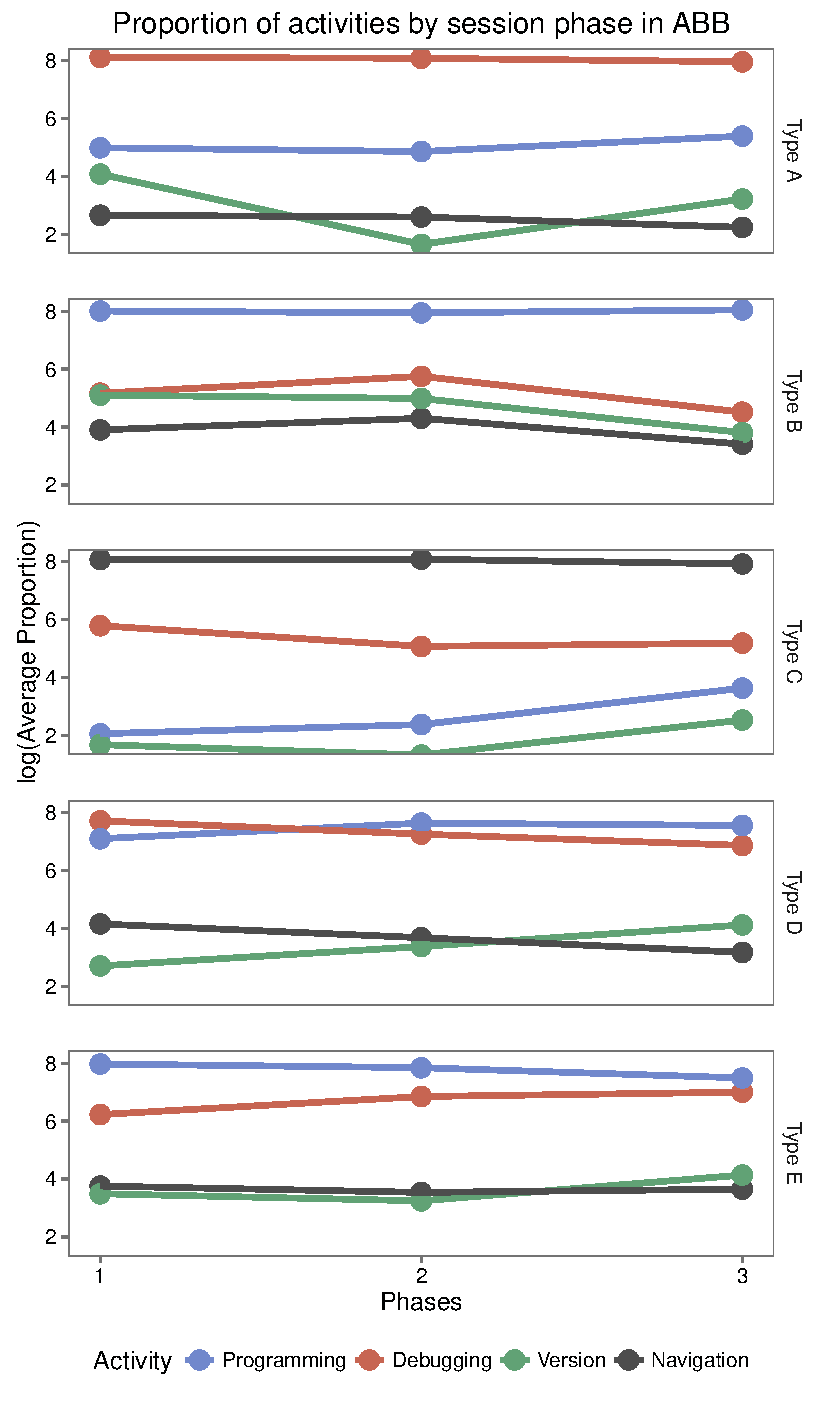
\includegraphics[width=0.35\textwidth]{Figures/ABB_phases_log}
	
	\caption{Cluster of sessions in UDC (left) and ABB (right).}
	\label{ABB_phases}
\end{figure*}

\section{Validation of the results}
To validate the results from the clustering of chunks and sessions we measure the Silhouette Width of the observations. The Silhouette Width is a number between 1 and -1; a value of 1 means that the observation is very well clustered and the contrary for a value of -1. If the value is close to 0 it means that the observation is between two different clusters.

In ABB the average Silhouette Average of the clusters of chunks is 0.55 and for UDC 0.38. This numbers represent a reasonable structural definition of the clusters. We can see in the Figure \ref{silhouette_chunks} the graphical representation of the silhouette of each cluster of chunks for ABB (right) and UDC (left). In average, the clusters in ABB are better defined but in both cases we can spot some observations wrongly clustered (negative values) that can also be outliers.

In the case of the clustering of sessions, we have an average silhouette of 0.35 for ABB and 0.40 for UDC, indicating also a reasonable structure but weaker than the structures in the chunks. This can be observed in the Figure \ref{silhouette_sessions}. In UDC a big number of the observations of the cluster Type C are outliers and the rest of the clusters are better defined. In ABB clusters Type A and C show good shape but the rest of the clusters have smaller averages.

Overall, we can see a clear pattern in the clustering of chunks and sessions. We believe the patters are strong enough to support our observations and the fact there are patters in the data. The data from ABB is stronger in this sense, probably due to the fact that it all comes from developers. In the other hand, the UDC data contains more variety of users and provokes a variety of activities and practices that are harder to cluster. 



\begin{figure}[!ht]
\centering		
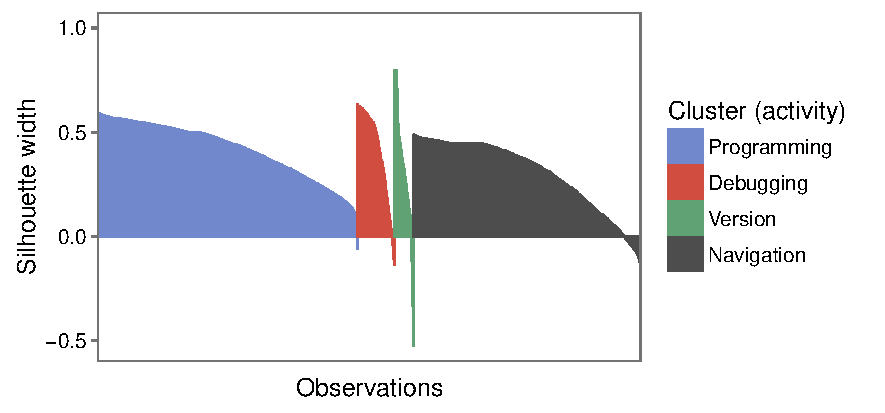
\includegraphics[width=0.4\textwidth]{Figures/UDC_silhouette_chunks}
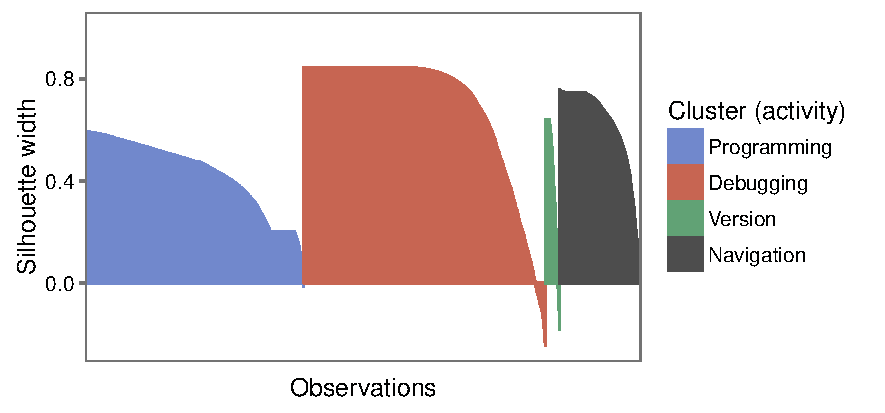
\includegraphics[width=0.4\textwidth]{Figures/ABB_silhouette_chunks}	
\caption{Silhouette analysis of the clustering of chunks for UDC (top) and ABB (bottom).}
\label{silhouette_chunks}
\end{figure}
	
	
\begin{figure}[!ht]
\centering		
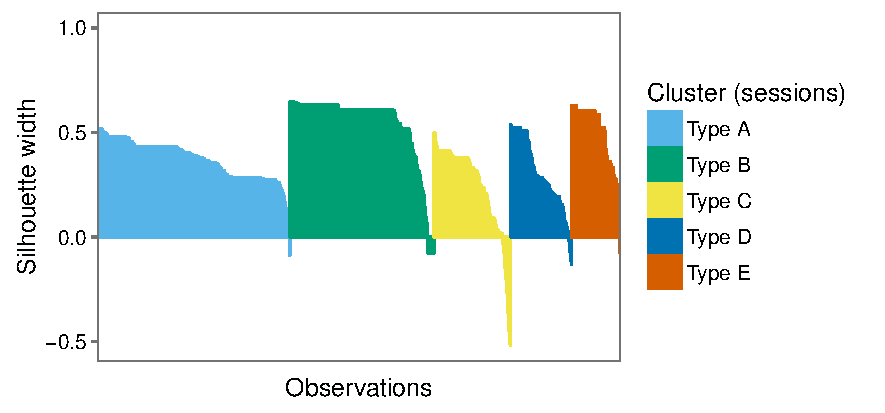
\includegraphics[width=0.4\textwidth]{Figures/UDC_silhouette_sessions}
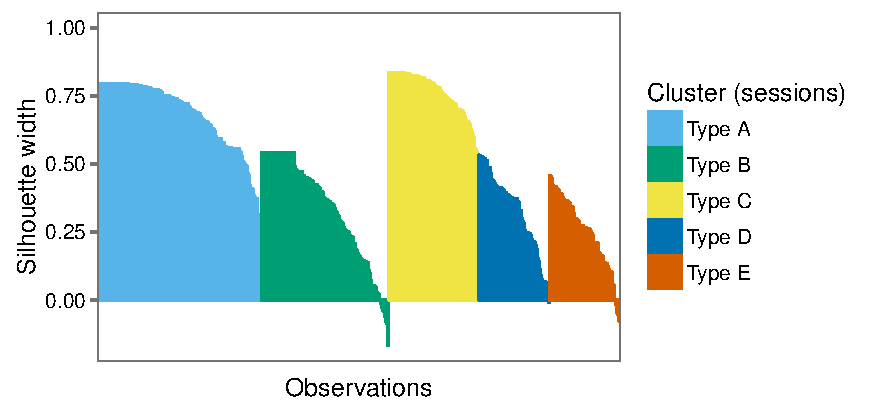
\includegraphics[width=0.4\textwidth]{Figures/ABB_silhouette_sessions}	
\caption{Silhouette analysis of the clustering of sessions for UDC (top) and ABB (bottom).}
\label{silhouette_sessions}
\end{figure}


\section{Conclusions}
In this paper we used clustering techniques to discover developers' activities and working patterns in usage data. The data came from two sources: the Usage Data Collector of Eclipse, with information of a variety of developers, and a second dataset extracted from Codealike that contains information of professional software developers from ABB. Now we proceed to answer the research questions established in the Introduction.

\textbf{RQ1: What kind of activities can be identified with interaction data?}
The first question was meant to discover what kind of activities we can find in the data according to executed events. Using small time frames of activity, we executed clustering techniques to find them. In the UDC data we found eight activities and in the ABB data only six. Five activities appear in both datasets (Debugging, Programming, Navigation, Versioning and Tool usage) and the rest are unique. The percentages also differ between datasets and it can be due to the different tools used to capture them and the kind of programmers of the samples. Most of this activities have been characterized in observational studies and we lack information to detect activities related to collaboration between developers and interactions outside of the IDE.

\textbf{RQ2: What working patterns during a session are commonly performed by developers?}

Once we had all the activities performed by the developers, we split every working session into three phases and cluster them to find patterns of activities. We found several centroids (patterns) but the most common correspond to working sessions were the programmer mostly performs programming activities, program comprehension or general activities (multitasking). These three kind of activities can be observed in both datasets. This patterns of activities can be related to types of working sessions observed in observational studies.

Overall, we conclude that it is possible to observe in usage data the performed by developers. The results we obtained can be matched to observations from observational studies and experiments, so that we gained confidence in using this kind of information to understand how developers work. However, due to the limitations with the datasets we are unable to observe other activities that occur outside the IDE and that cover a considerable part of a developer day-to-day work. It may be possible in the near future to have better programming tools that learn from the activities of the user and offer assistance in common challenges and problems that developers face in a daily basis, and be able to mutate according to the circumstances.



\section*{Acknowledgment}
The completion of this work could not have been possible without the collaboration with David C. Shepherd, Senior Principal Scientist at ABB Corporate Research, who provided the ABB dataset previously described.


\bibliographystyle{IEEEtran}
% argument is your BibTeX string definitions and bibliography database(s)
\bibliography{IEEEabrv,mybib}



% that's all folks
\end{document}


